\documentclass{beamer}
\usepackage{apacite}
\usepackage{background,quoting,setspace}
\usepackage[utf8]{inputenc}
\usepackage[T1]{fontenc}
\usepackage[portuguese]{babel}
\usepackage{graphicx}


\logo{

\includegraphics[width=2.5cm]{logo.png}
}

\setbeamertemplate{background canvas}{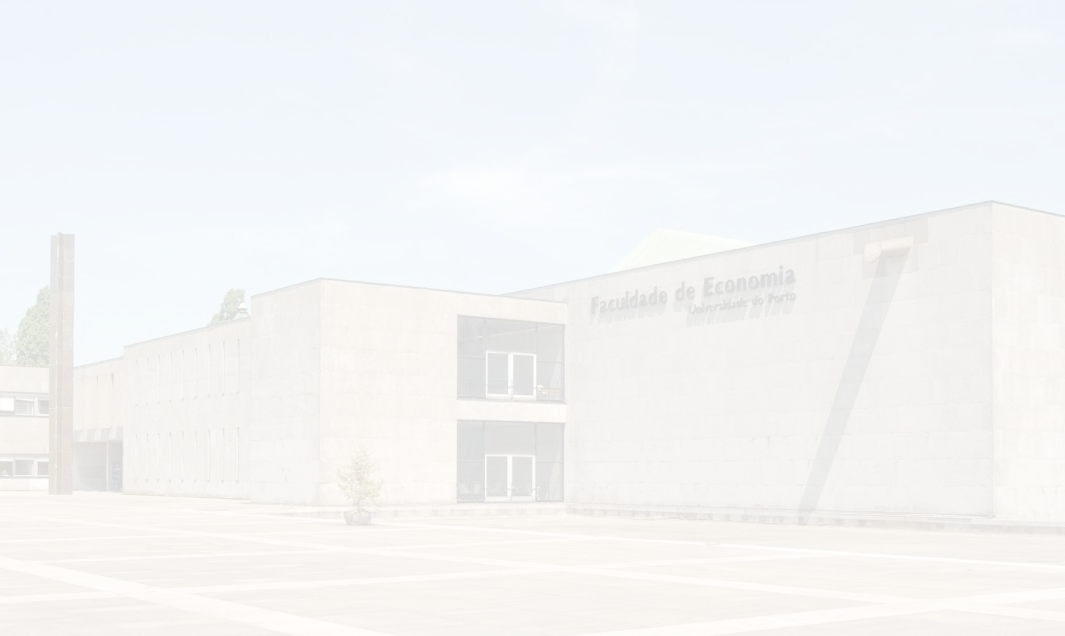
\includegraphics[width=\paperwidth,height=\paperheight]{fep.png}}

\author{Gustavo de Oliveira Vital \and Miguel Peixoto Lages \\ Rodrigo Gomes Silva}
\date{\today}
\title{On The Effectiveness of Macroprudential Policy}
\institute{FEP - Faculdade de Economia do Porto}
%\bibliography{bib}




\begin{document}

%---------------------------------------

\begin{frame}
\maketitle
\end{frame}


%---------------------------------------

\begin{frame}
    \tableofcontents
\end{frame}


\begin{frame}{Introduction}
    \section{Introduction}
    Como dito por \cite{ampudia2021effectiveness}
\end{frame}

\begin{frame}{A general framework for macroprudential policy}
    \section{A general framework for macroprudential policy}
\end{frame}

\begin{frame}{Macroprudential policy and financial stability: theory}
    \section{Macroprudential policy and financial stability: theory}
\end{frame}

\begin{frame}{Macroprudential policy and financial stability: empirical evidence}
    \section{Macroprudential policy and financial stability: empirical evidence}
\end{frame}

\begin{frame}{Financial stability and growth}
    \section{Financial stability and growth}
\end{frame}

\begin{frame}{Conclusion}
    \section{Conclusion}
\end{frame}


\begin{frame}[allowframebreaks]{References}
    \section{References}
    \nocite{ampudia2021effectiveness}
    \bibliographystyle{apacite}
    \bibliography{bib}
\end{frame}
\end{document}
